\scanpage{68}
% archive sheet number: 67
% Two long diagonal strokes cancel this draft. Unfilled sign slots are left as spacing.
\deleted{under the conditions considered a) b) $\quad)$ $\quad)$, $B$ flat over $A$ and with finite residue field extension,}
\[
\deleted{\text{\uuline{R}}(A)\quad\text{and}\quad\text{\uuline{R}}(B\otimes k)\ \text{geometric}\quad\text{imply}\quad\text{\uuline{R}}(B).}
\]
% Two isolated nonalphabetic dark hook-like marks in the left margin, below point; function/origin uncertain.
\margin{\figure{\begin{tikzpicture}[x=.8cm,y=.8cm]
\draw[line width=.55pt] (0,0) .. controls (.12,-.02) and (.25,-.01) .. (.33,.02) -- (.29,.19);
\draw[line width=.75pt] (1.35,-.10) -- (1.64,-.13) -- (1.56,.15);
\end{tikzpicture}}}
\deleted{The additional condition that we have just pointed out for \uuline{R} is satisfied in all the examples considered in 7.5.3., except for (vii), where it fails. Indeed, one can (even \deleted{over a field} for a curve $Y$ over an algebraically closed field $k$ of arbitrary characteristic) give examples of an étale morphism $f\colon X\quad Y$, and of a point $x$ of $X$ such that $Y$ is integral at $y=f\rlap{\(x\)}(x)$, but $X$ is not at $x$.\handwritten{/} This would perhaps be the moment to give the example (also pointed out in 6.15.7. and which is used again $X$ times): one takes a curve with an \unsure{o|\rlap{r}o}\unsure{\rlap{u}r|r}dinary double point, and one glues together two copies of the normalization \unsure{d|of} so as to have an étale curve $X$ over $Y$. An analogous example with a \mbox{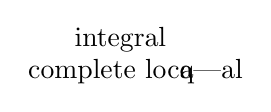
\begin{tikzpicture}[baseline=(base.base)]
\node[inner sep=0] (base) {\uline{complete} loc\unsure{\rlap{q}a|a}l};
\path (base.north west) -- coordinate[pos=.43] (ins) (base.north east);
\node[anchor=south,inner sep=0,yshift=.08cm] at (ins) {\inserted{integral}};
\end{tikzpicture}} ring, hence unibranch, but in this instance not geometrically unibranch, is given by $\overset{\textstyle\inserted{A=}}{\text{\uuline{R}}}\ X,Y\quad/(X^{\handwritten{2}}+Y^{\handwritten{2}})$. \deleted{If $X$ is its spectrum} Then $A\otimes_{\underline{R}}\underline{C}$ is étale over $A$, but not integral. These examples, which one seems to encounter for the first time in connection with 6.15.7. could perhaps be moved up to that place.\handwritten{/} It is however p\rlap{o}lausible that \deleted{the statement which} the answer to the following question is affirmative :}

\deleted{Let $A\quad B$ be a local homomorphism of noetherian local rings, $B$ flat over $A$, $B\otimes_A k\handwritten{/}k$ geometrically integral, $A$ \deleted{excellent (for example complete)} geometrically unibranch (NB one can reduce to the case: $A$ normal). If $A$ is moreover excellent (say complete), then is $B$ integral ?}

\deleted{The answer is affirmative when the residue field $k$ of $A$ is of characteristic 0, as we shall see in number\textsuperscript{\uline{o}} 7.9. using the\deleted{é} resolution of singularities of Hironaka, or when $B$ is essentially of finite type over $A$ (reference $\qquad$). B\rlap{i}u\rlap{a}t \mbox{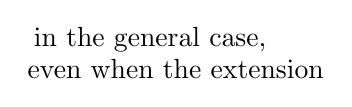
\begin{tikzpicture}[baseline=(base.base)]
\node[inner sep=0] (base) {even when the extension};
\node[anchor=south west,inner sep=0,yshift=.08cm,xshift=.08cm] at (base.north west) {\inserted{in the general case,}};
\end{tikzpicture}} of residue fields is trivial, $A$\deleted{\unsure{s|x}} and $B$ complete, \deleted{the technique \unsure{dévis}} we do not know whether the answer is affirmative. We have however a partial result below.}
